\chapter{Kernel density estimation}
\section{Bandwidth and Kernel function}
In this chapter we are dealing with marks secured by students in various subject, along with  explanatory variables about the students viz., gender, ethnicity etc.. For our analysis for student's performance together with scores in mathematics, reading and writing tests, we consider students attendance for the test preparation course. We drop rest of the variables. Following is the sample for first few entries of the dataset;

\begin{table}[ht]
\centering
\begin{tabular}{llrrr}
  \hline
 & test preparation course & math score & reading score & writing score \\ 
  \hline
1 & none &  72 &  72 &  74 \\ 
  2 & completed &  69 &  90 &  88 \\ 
  3 & none &  90 &  95 &  93 \\ 
  4 & none &  47 &  57 &  44 \\ 
  5 & none &  76 &  78 &  75 \\ 
  6 & none &  71 &  83 &  78 \\ 
  7 & completed &  88 &  95 &  92 \\ 
  8 & none &  40 &  43 &  39 \\ 
  9 & completed &  64 &  64 &  67 \\ 
  10 & none &  38 &  60 &  50 \\ 
   \hline
\end{tabular}
\end{table}

In this exercise we are suppose to implement kernel density estimation. The data entries i.e. math score are integers variables. Kernel density estimation help us visualize the “shape” of data, even though its discrete. Essentially it is sort of continuous replacement for the discrete histogram. Kernel estimation uses a weighted sum of observations dependent on their distance from the variable. The precise definition is as follows, for the given data $X_1, X_2,..., X_n$, a kernel density estimator is 
$$\widehat{f}_{n,h}(x)= \frac{1}{nh}\sum_{1 = j}^n K\left(\frac{x-X_j}{h}\right), \: x\in \RR .$$ 
where $K: \RR \rightarrow \RR$, such that $\int_{-\infty}^{\infty}K(x)dx=1$ is known as kernel and $h>0$ is called the bandwidth. $h$ is smoothing parameter which basically governs how many distinct observations are taken into account around certain location. Thus it has a strong influence on the resulting estimate. Examples of some classical kernels is illustrated below in Figure \ref{fig:types_kernels8}.
    
\begin{figure}[thb]
\centering
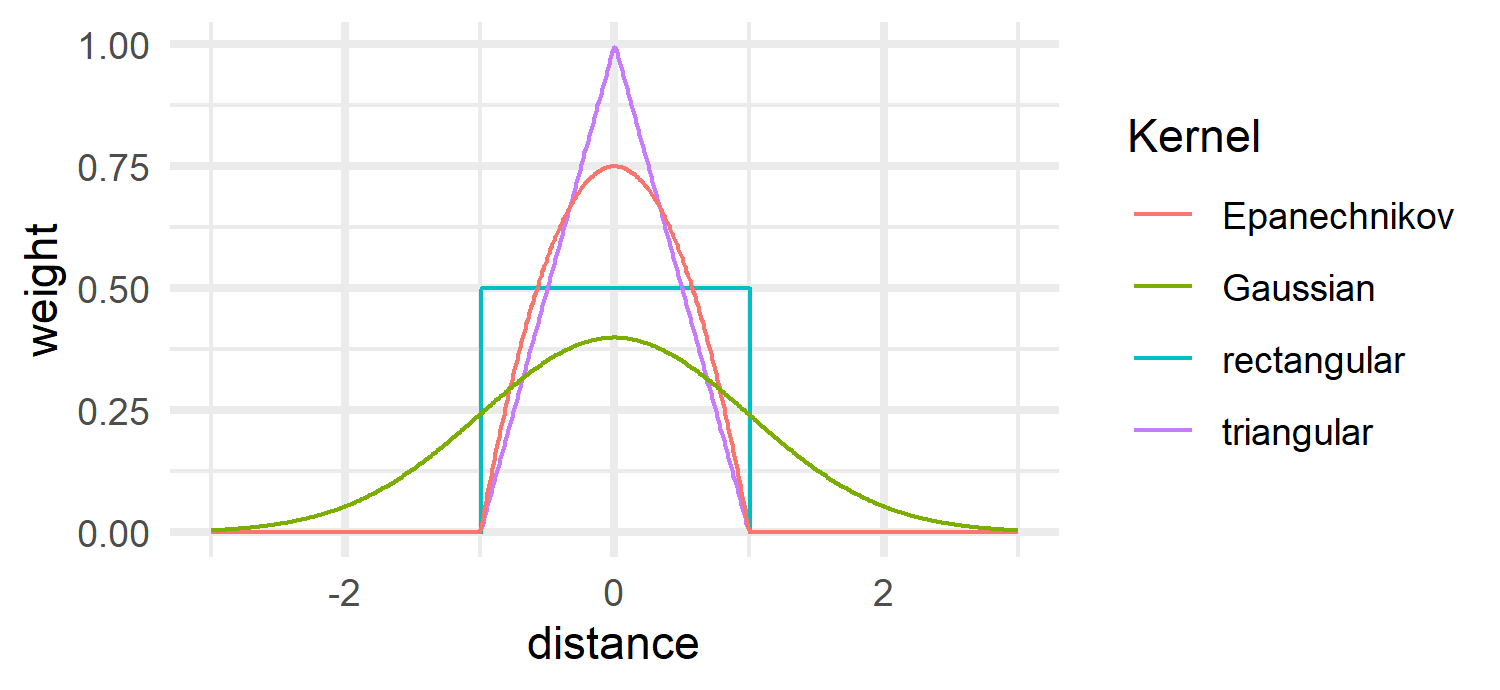
\includegraphics[width=0.75\textwidth, keepaspectratio]{ex8/types_kernels.png}
\caption{Classical examples of kernels often used for density estimation. }
\label{fig:types_kernels8}
\end{figure}

To visualise and examine the influence of the choice of bandwidth and kernel we have considered the math score variable from the data. First we fit a kernel density with different bandwidths using the Epanechnikov kernel (See Figure \ref{fig:diff_bandwidth8}) and then use different kernels with a fixed bandwidth Figure\ref{fig:diff_ker8} ). We can clearly see the influence of the choice of bandwidth.  The estimated curves get smoother with higher and higher $h$. For bandwidth $= 2$ it fluctuates highly. 
For the values  of $h$ between $5$  and  $12$ seems reasonable where as for for  higher values, like $30$ density curve gets  too  smooth and it certainly does not represent the shape of the data distribution anymore. Since, visually it appears that the most reasonable bandwidth lies between $5$ and $12$, I have fixed $h= 8$ for the next analysis (See Figure \ref{fig:diff_ker8}). We will now compare different kernels choices with a fix bandwidth $h= 8$.

\begin{figure}[tbh]
\centering
\begin{subfigure}[c]{\textwidth}
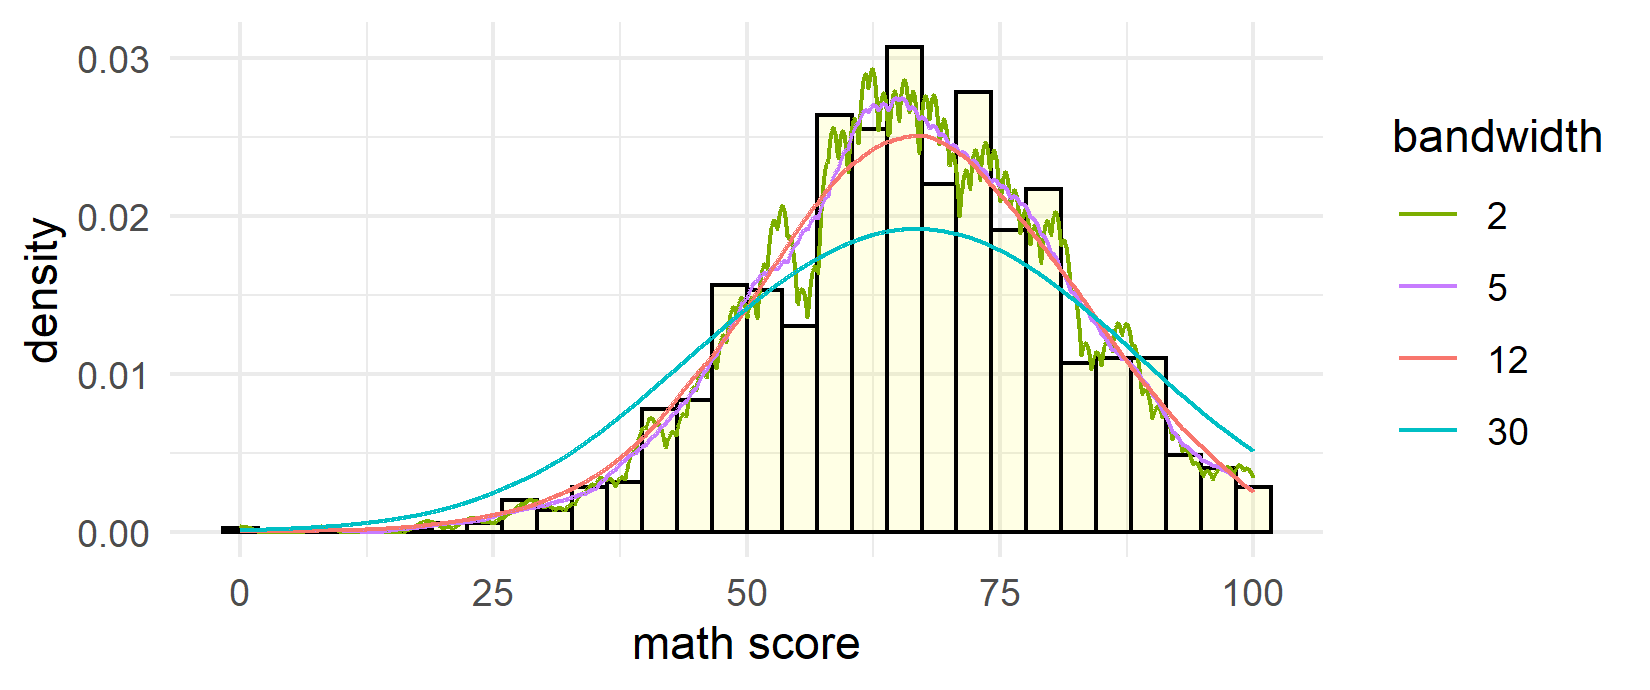
\includegraphics[width=0.93\textwidth, keepaspectratio]{ex8/diff_bandwidths.png}
\subcaption{Epanechnikov kernel with different bandwidths.}
\label{fig:diff_bandwidth8}
\end{subfigure}
\begin{subfigure}[c]{\textwidth}
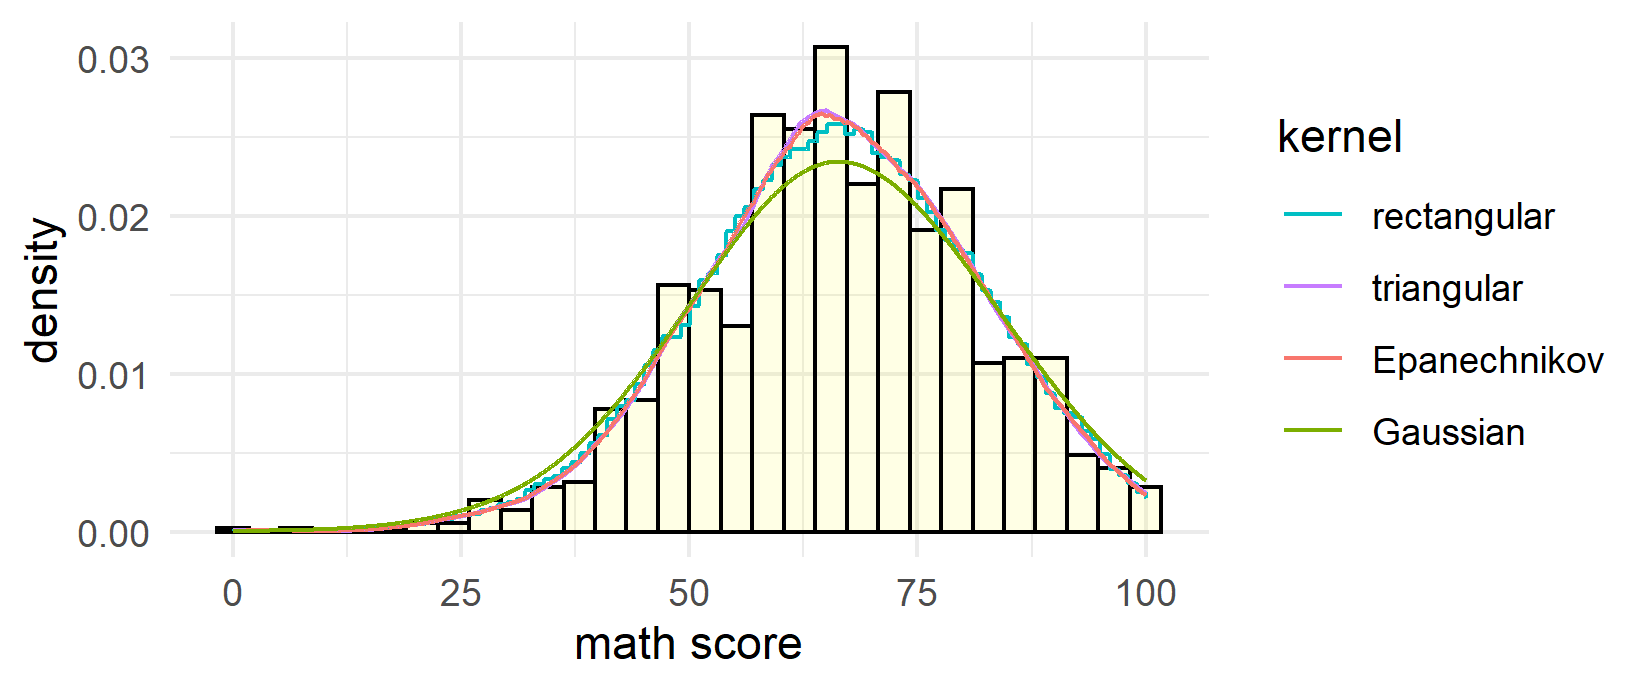
\includegraphics[width=0.98\textwidth, keepaspectratio]{ex8/diff_ker.png}
\subcaption{Different kernels with fixed bandwidth $h=8$.}
\label{fig:diff_ker8}
\end{subfigure}
\caption{Kernel density estimations for the math score  (first plot) and kernels (second plot).}
\label{6fit}
\end{figure}

%Comment on the effect of the bandwidth and of the kernel function on kernel density estimators
If we observe closely Figure \ref{fig:types_kernels8}, we can see that, the different shapes of the kernels shows how observations with certain weights at different distances influence the height of the density estimation at specific points. Therefore, the shape and some basic properties of the resulting density estimations depend highly on the choice of the kernel. The rectangular kernel for example will always result in a piece-wise constant estimation, which is not continuous.  The triangular kernel will give us a piece-wise linear density and the Gaussian kernel will result in smooth estimations. In Figure \ref{fig:diff_ker8} we can see that for the rectangular kernel the result is a step function, where as the rest of the kernels seem smoother. But as mentioned before the curve for the triangular kernel is piece-wise linear. Rectangular, triangular and Epanechnikov look quite similar with respect to the shape of the overall distribution. The Gaussian kernel produces a flatter curve that puts more mass to the tails. This might be because, of the differences in support of kernels. The support of the Gaussian kernel $\RR$ and its $ [ -1,1] $ for the other kernels. Thus, as we can also see in Figure \ref{fig:types_kernels8} Gaussian kernel puts more mass to the tails.

\section{Cross validation for optimal bandwidth}  
Now we want to consider a more formal approach to examine the best bandwidth. Above we just did a graphical examination. To get the best fitting curve a common approach is trying to minimise the mean integrated square error (MISE) for the estimator $\hat{f}_{n,h}(x)$ of $f(x)$, which is given by $$MISE(\hat{f}_{n,h})=E\left[\int\left(\hat{f}_{n,h}(x)-f(x)\right)^2dx\right].$$ Because the real $f$ is unknown one minimises an unbiased estimator of the $h$-dependent part of the MISE, called the cross-validation criterion: $$CV(h)=\int\left(\hat{f}_{n,h}(x)\right)^2dx-\frac{2}{n(n-1)h}\sum_{i=1}^{n} \sum_{j\neq i} K\left(\frac{X_j - X_i}{h}\right).$$
\begin{figure}[!tb]
\centering
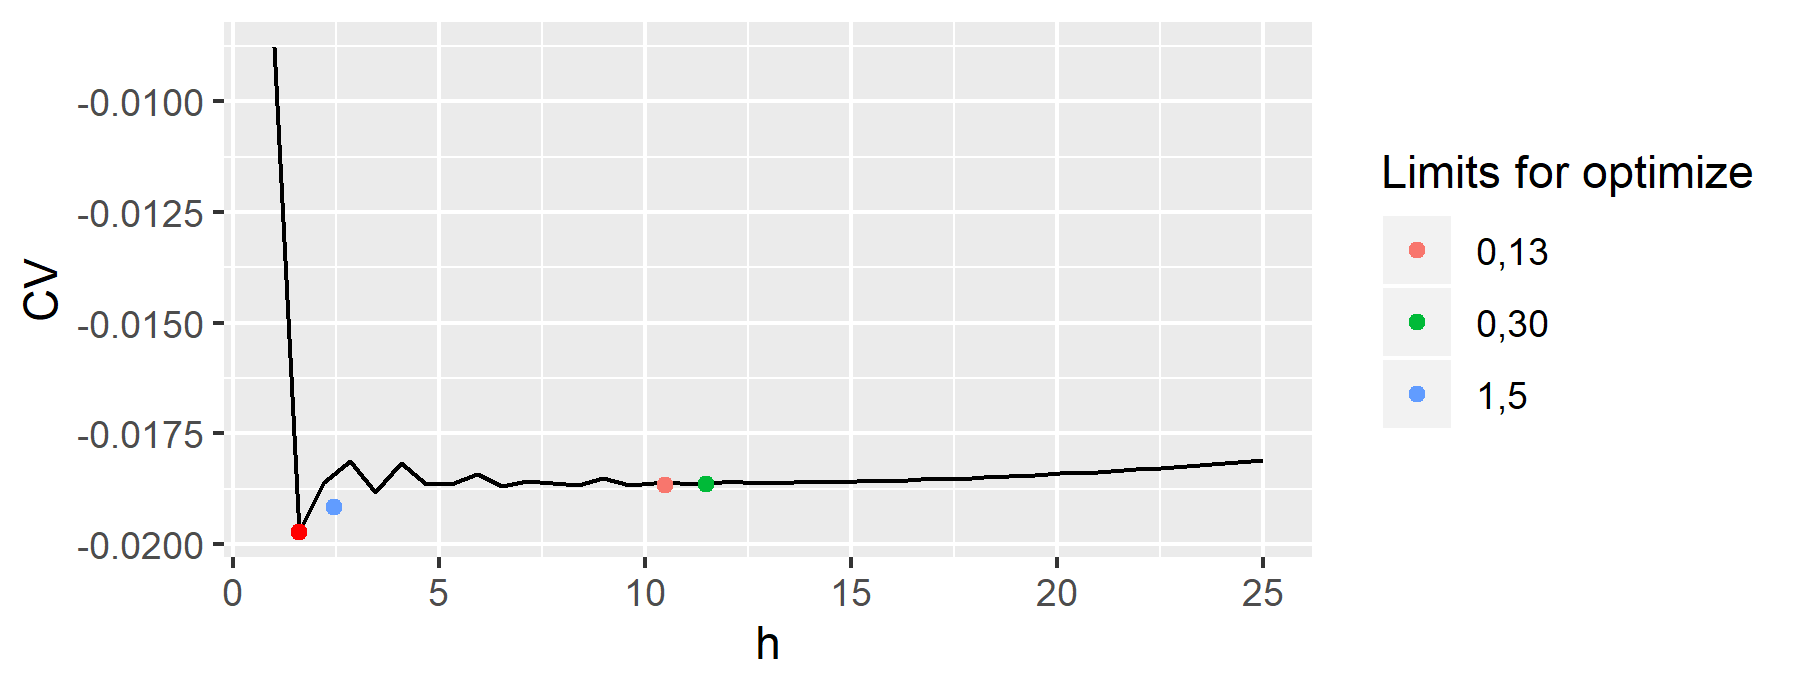
\includegraphics[width=0.9\textwidth, keepaspectratio]{ex8/CV1.png}
\caption{CV values for 40 different bandwidths. Red point shows minimum of the curve. Other points show the results for the \texttt{optimize} function in R with different limits (see legend).}
\label{6CV1}
\end{figure} 

Implementing a function computing the CV for a given estimation we can use the minimising $h_{CV}=\argmin _{h>0} CV(h)$.
Afterwards we compared the results with the functions \texttt{bw.ucv} and \texttt{bw.bcv} of the package \texttt{density}, which compute the optimal bandwidth for an unbiased (\texttt{ucv}) or biased (\texttt{bcv}) CV implementation for Gaussian kernels. 
Therefore I used the Epanechnikov kernel as well as the Gaussian kernel in my implementation to compare all results for the maths score. To find the minimizer of my function, I used the R function \texttt{optimize}. Before comparing the optimisation of my own CV function a little note about the disadvantages of using \texttt{optimize} here is important. 
To get a first idea of the shape of CV for different $h$ as a curve I took 40 equidistant points in the interval $[1,25]$ - because it seemed as a (maximal) reasonable region for bandwidths in this case -  and computed CV there. Afterwards I took the minimum out of this observations as first reference point ($h=1.62$). After using the R implemented optimisation with limits 0 and 30, I was surprised by the result ($h=11.50$). As \texttt{optimize} just searches for local minima and starting points for the iteration are chosen as a golden section distance between the given limits, the result also depends highly on those borders. Obviously CV is a strongly fluctuating function as I got different results for every trial, none of them was near the first, say, 'scanned minimum'. Figure \ref{6CV1} shows the results. All in all, without an analytical examination of CV as a function one cannot be sure to really found the optimal bandwidth or even to be close to it. In the following I won't discuss this issue any more- I will use a combined strategy by first scanning the interval $[1, 20]$ with 40 points to get the area of small values visually and by taking the minimum. Afterwards I will use \texttt{optimize} limited to this region to get a local minimum. This should in total result in a somehow precise and at least acceptable minimum. The results for all three tests and the different methods are shown together in Table \ref{6table}. For the math score and the best bandwidth with a Epanechnikov kernel we use the above optimal $h=1.62$. 
\begin{figure}[p]
\centering
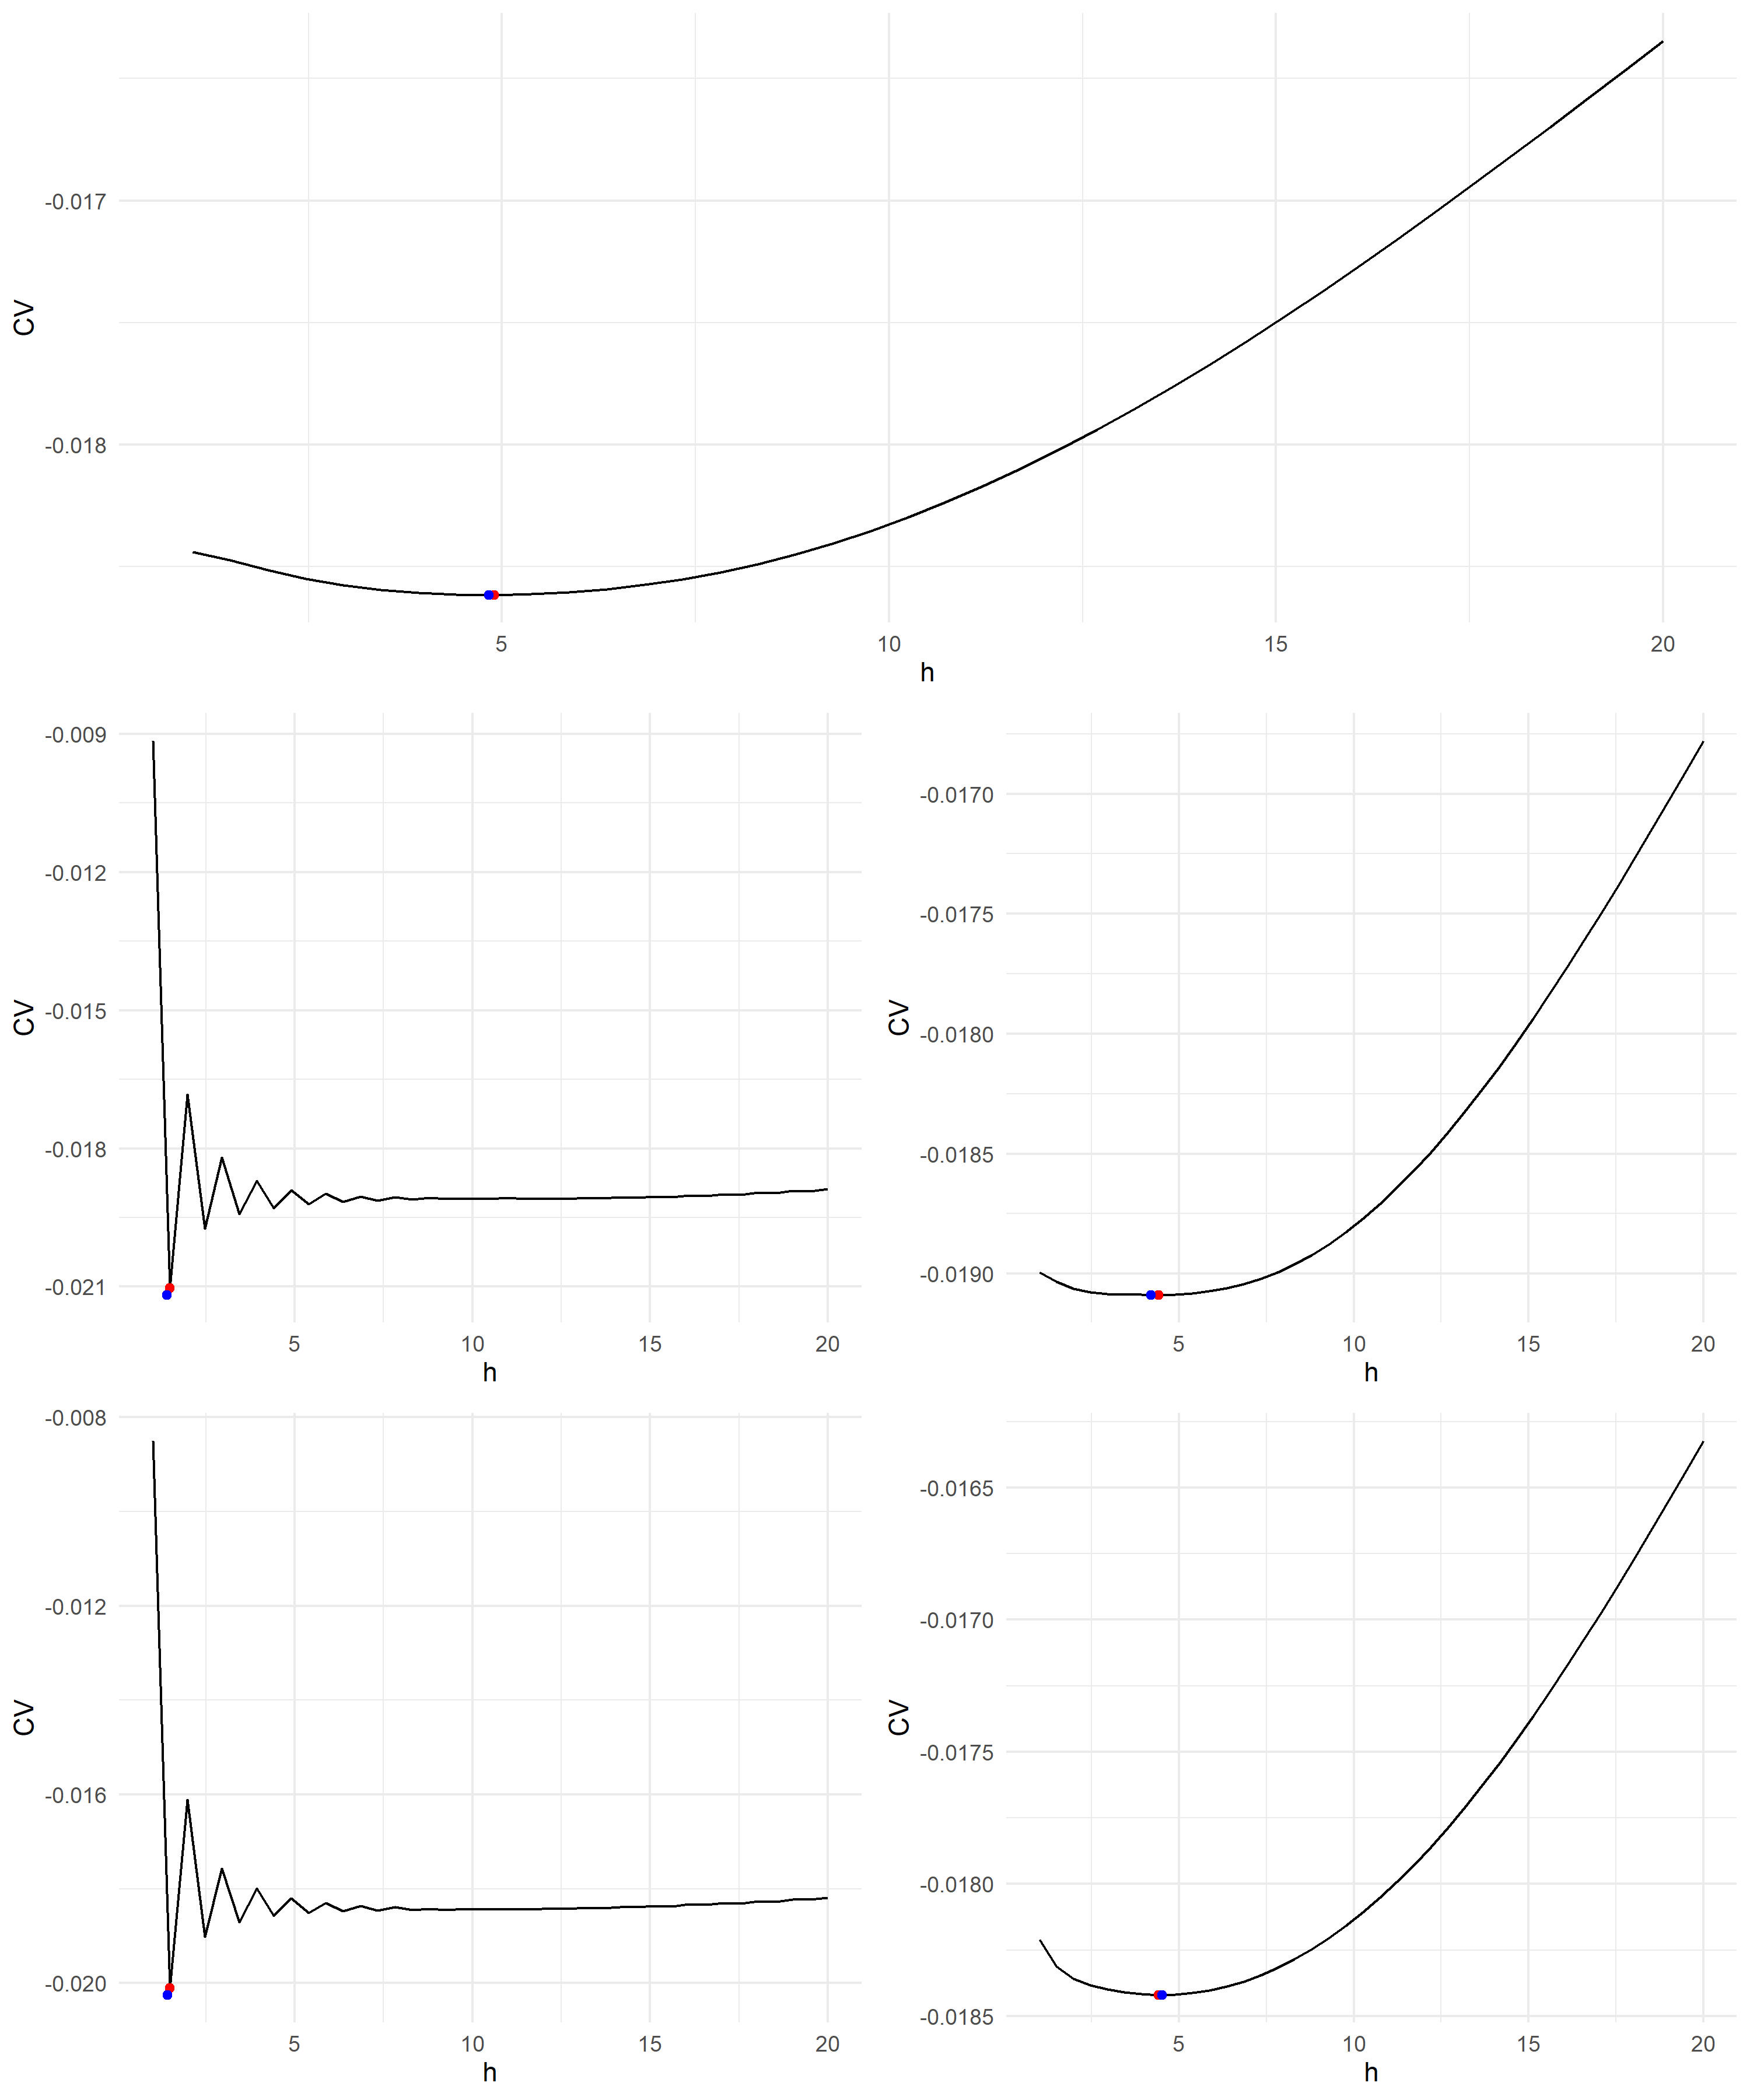
\includegraphics[width=\textwidth, keepaspectratio]{ex8/CVplots.png}
\caption{CV against $h$ for math score and Gaussian kernel (first row), reading score (second row) and writing score (third row). Last two for Epanechnikov  kernel (left) and Gaussian kernel (right)}
\label{6CVs}
\end{figure}

First, observe (see Figure \ref{6CVs}) that for the Gaussian kernel the problem of fluctuating CV function is not that worse but the usage of the \texttt{optimize} function still improves the optimal bandwidth a bit. For the Epanechnikov kernel we have the same problem for every test. All in all the CV curves look very similar for math, reading and writing score. Therefore we get quite similar results for optimal bandwidths. As expected the values of my own optimisation for the Gauss kernel are similar to those of the R functions but differ from the optimal bandwidth for the Epanechnikov kernel. For every score the resulting CVs just differ on the presented scale between the kernels where always the Epanechnikov kernel gives a better result. Therefore we use this bandwidth an the Epanechnikov kernel for the last part of the exercise. 

\begin{table}[!t]
\centering
\begin{tabular}{lrrrrrrrr}
  \hline
 & \multicolumn{2}{r}{Epa} &  \multicolumn{2}{r}{Gau}&  \multicolumn{2}{r}{\texttt{bw.bcv}}&  \multicolumn{2}{r}{\texttt{bw.ucv}} \\  
\hline
 & h & CV & h & CV & h & CV & h & CV \\ 
  \hline
math & 1.62 & -0.0197 & 4.83 & -0.0186 & 4.26 & -0.0186 & 4.65 & -0.0186 \\ 
  reading & 1.41 & -0.0212 & 4.19 & -0.0191 & 4.40 & -0.0191 & 3.77 & -0.0191 \\ 
  writing & 1.41 & -0.0203 & 4.52 & -0.0184 & 4.18 & -0.0184 & 4.28 & -0.0184 \\ 
   \hline
\end{tabular}
\caption{Optimal bandwidths $h$ and corresponding CV for math, reading and writing score and different methods. First two columns are optimum of self-written function with Epanechnikov kernel (Epa) and Gaussian kernel (Gau) respectively, last two columns with R function in the package \texttt{density}.}
\label{6table}
\end{table}


\section{Comparison of groups}
Now we use the kernel density estimation for a comparison of those students attending a preparation course and those that did not. Therefore we fit a curve for both groups using the optimal bandwidth we got in the previous examinations and the Epanechnikov kernel. For the bandwidth we use a common value equal to the mean of the three optimal bandwidths (this is just for a simplification of the code and does not change the results crucially). 

The result is shown in Figure \ref{6groups}. I decided to plot the histograms above each other, so that there is no confusion about the positioning and because one can still distinguish the bars with just two groups. We see that for the math score the whole distribution of scores is not changed very much in the shape but just shifted to the right, i.e. to better grades. For the other two scores we can recognise that the distribution of students with the preparation course is a bit more left skewed. This is just slightly visible for the reading score and a bit more distinct for the writing score. This is probably due to the fact that the student get better in total but the limit of the score is at 100. Psychologists call this effect \textit{ceiling effect}. This is maybe also the reason why the distribution has a smaller variation, especially for the writing score again. Summing up, we recognize better performance of students doing a preparation course. This is especially visible for the writing score. Apparently, one cannot train maths as easily as writing.
\begin{figure}[!t]
\centering
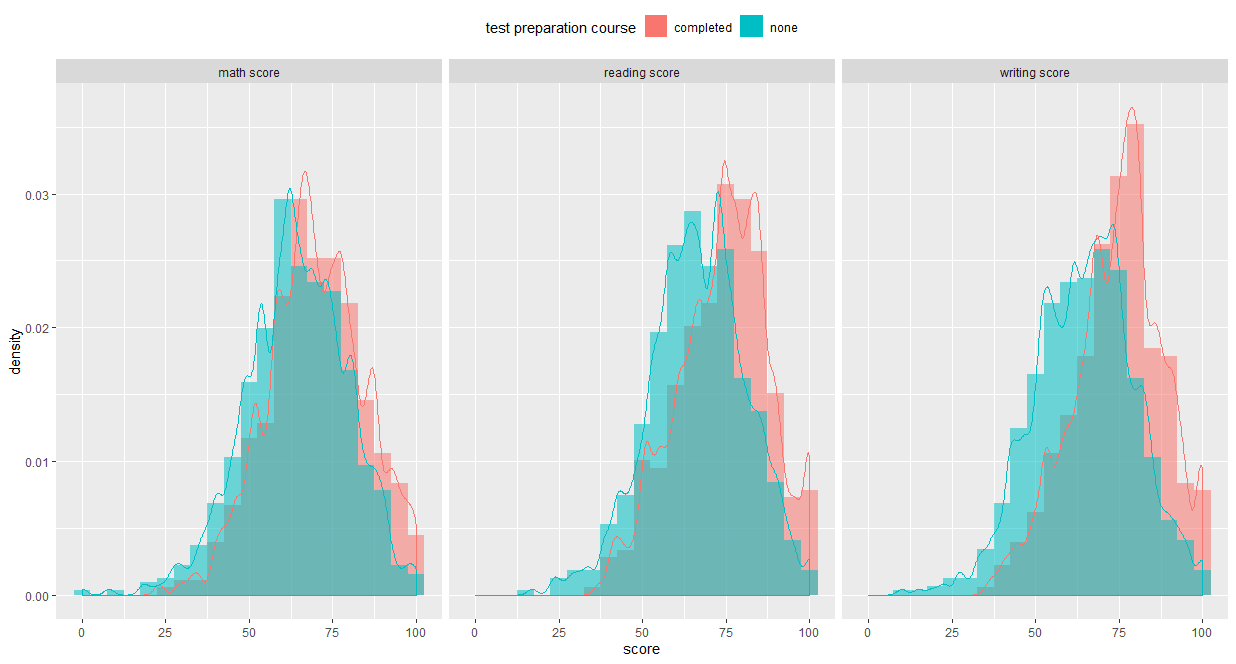
\includegraphics[width=\textwidth, keepaspectratio]{ex8/groups.png}
\caption{Histogram and kernel density estimate for two groups of students in different colors and the three scores, math (left), reading (middle) and writing (right).}
\label{6groups}
\end{figure} 
